\section{\texorpdfstring{Further information for baryonic \Zprime Model}{Further information for baryonic Z' Model}}

\subsection{Cross-section scaling}

The dependence of the cross section of the $pp \rightarrow H\chiDM\bar{\chiDM}+X$ process 
on $g_{h \Zprime \Zprime}$ is shown in Figure~\ref{fig:vectorXSdeps}. 
The curves have been fit to second-order polynomials, where $y$ is the cross-section
and $x$ is the coupling $g_{h \Zprime \Zprime}$. 

For $m_{med} = 100$~\gev, the fit function is 
$$y = -0.12 - 3.4\times10^{-3}x + 2.7\times10^{-4}x^2$$.
For $m_{med} = 1$~\tev, the fit function is 
is $$y = 0.0012 - 2.4\times10^{-7}x + 1.5\times10^{-7}x^2$$,

\be
y = -0.12 - 3.4\times10^{-3}x + 2.7\times10^{-4}x^2.
\ee
For $\mMed = 1$ TeV, the fit function is 
is:

\be
y = 0.0012 - 2.4\times10^{-7}x + 1.5\times10^{-7}x^2.
\ee

\begin{figure}[hbpt!]
	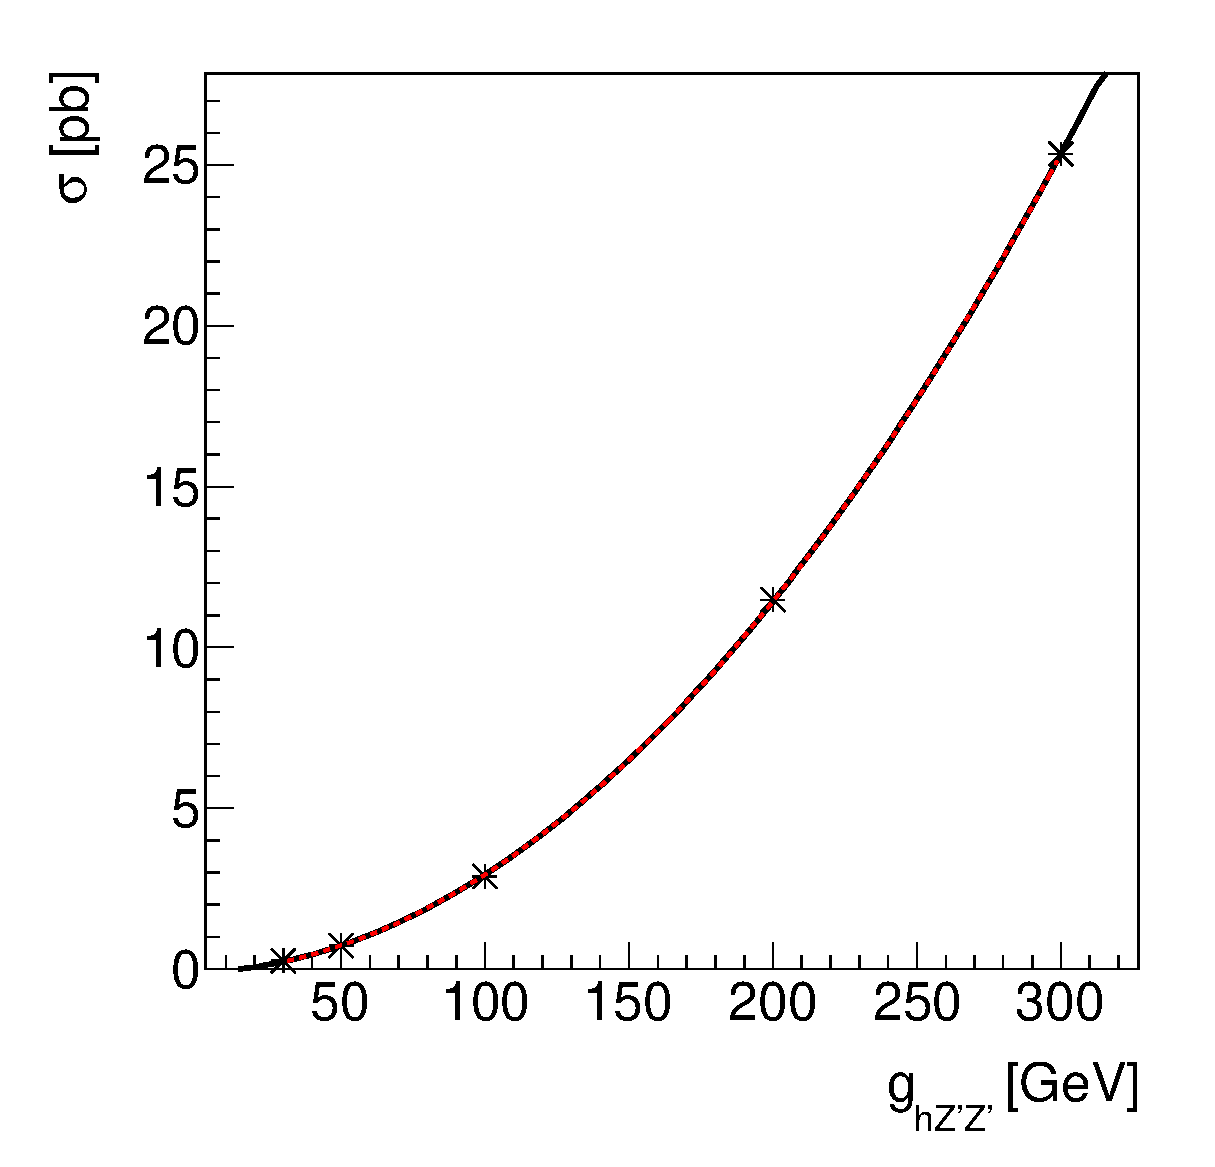
\includegraphics[width=0.99\linewidth]{figures/EW/monoH/zprime_xs_med_100}\\
	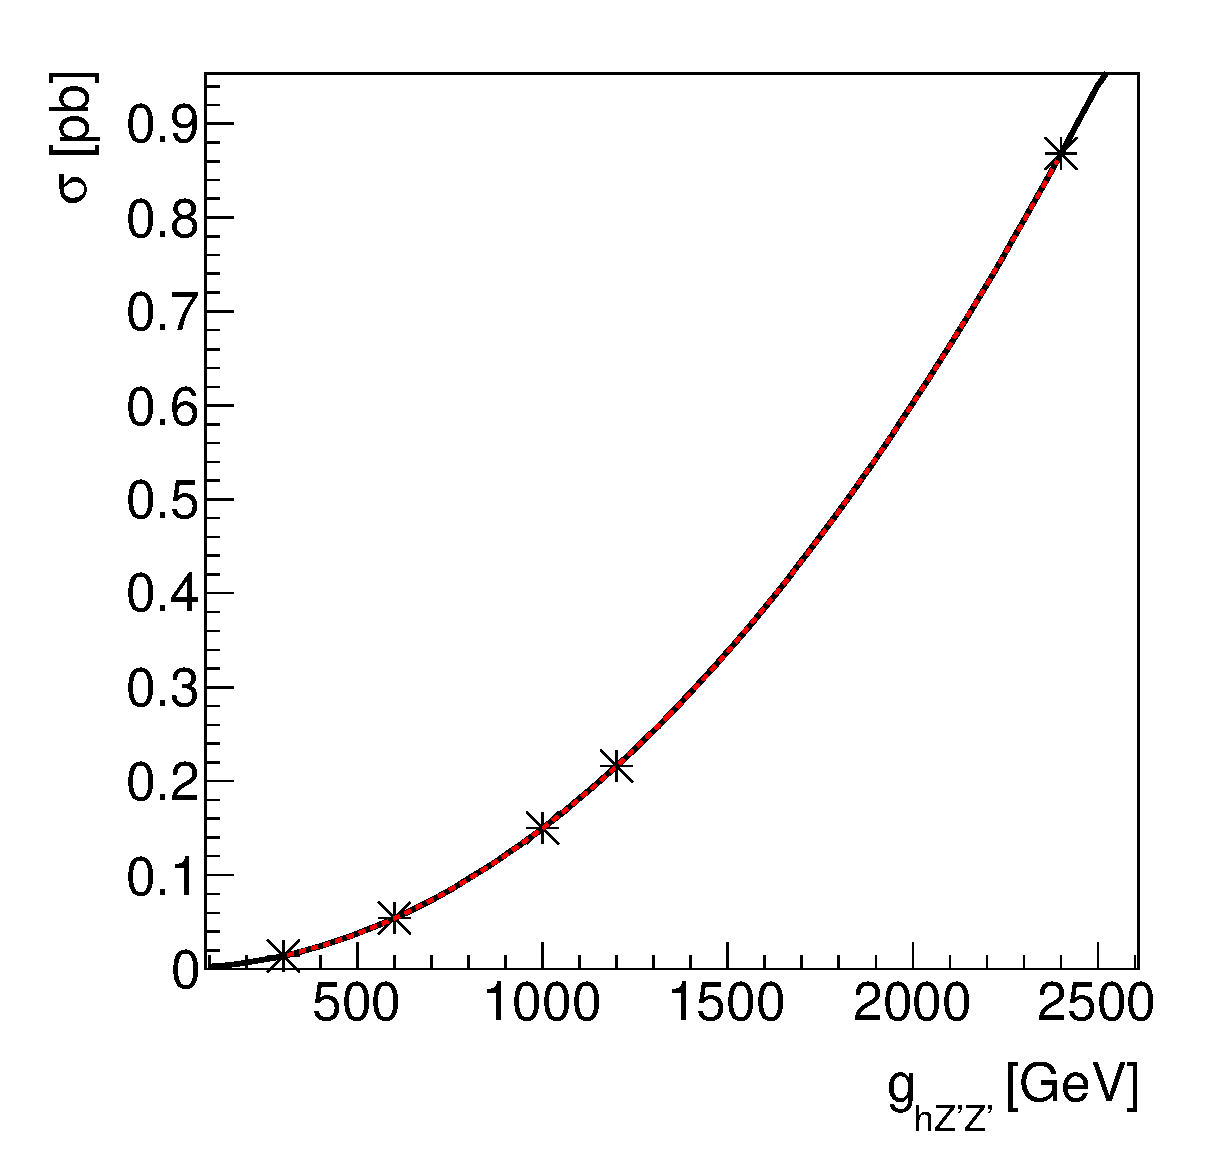
\includegraphics[width=0.99\linewidth]{figures/EW/monoH/zprime_xs_med_1000}
	\caption{Cross section of the $pp \rightarrow H\chiDM\bar{\chiDM}$ process as a function of 
		$g_{h \Zprime \Zprime}$ for $m_{\Zprime} = 100$~\gev (left) 
		and $m_{\Zprime} = 1$~\tev (right). The fit functions are shown in the text. 
		\label{fig:vectorXSdeps}}
\end{figure}




\section{Minimal mediator width in \schannel exchange}

Tables\,\ref{tab:widthV} and \ref{tab:widthA} give the $\Gamma_{\rm{min}}/\mMed$ ratio for the parameter grid proposed in Section\,\ref{sec:monojet_V} for vector and axial-vector \schannel models, respectively. The numbers range from $\sim0.02$ in the off-shell Dark Matter production regime at $2\mDM>\mMed$ to $\sim0.06$ in the on-shell regime for heavy mediators where all coupling channels contribute.

For the parameter grid for scalar and pseudo-scalar mediator exchange in \schannel proposed in Section\,\ref{sec:monojet_scalar}, the $\Gamma_{\rm{min}}/\mMed$ ratio is given in Tables\,\ref{tab:widthS} and \ref{tab:widthP}, respectively. In the on-shell production regime, the ratio is $\sim0.04$. Very narrow resonances with $\Gamma_{\rm{min}}/\mMed<0.001$ correspond to the mass points where Dark Matter is produced off-shell. Note that the loop-induced contribution from gluons is ignored in the width calculation.


\begin{table}
\centering
\resizebox{\textwidth}{!}{
\begin{tabular}{| l |r r r r r r r r r r|}
\hline
\multicolumn{1}{|c|}{\mDM/\gev} & \multicolumn{10}{c|}{\mmed/\gev} \\
              &         10  & 20 & 50 & 100 & 200 & 300 & 500 &         1000  &                 2000   &         10000  \\
\hline
\hline
   1 & 0.049  & 0.051  & 0.051  & 0.051  & 0.051  & 0.051  & 0.056  & 0.056  & 0.056  & 0.056  \\
  10 & 0.022  & 0.024  & 0.054  & 0.052  &        &        &        &        &        & 0.056  \\
  50 & 0.022  &        & 0.025  & 0.025  & 0.055  & 0.053  &        &        &        & 0.056  \\
 150 & 0.022  &        &        &        & 0.025  & 0.025  & 0.061  & 0.058  &        & 0.056  \\
 500 & 0.022  &        &        &        &        &        & 0.029  & 0.030  & 0.060  & 0.057  \\
1000 & 0.022  &        &        &        &        &        &        & 0.030  & 0.030  & 0.057  \\
\hline
\end{tabular}}
\caption%[][5cm]
{Minimal width of the vector mediator exchanged in \schannel divided by its mass, assuming $\gq=0.25$ and $\gDM=1$. The numbers tabulated under $2\mDM=\mMed$ correspond to the width calculated for $\mMed-5$~\gev.}
\label{tab:widthV}
\end{table}
\vspace{4cm}

\begin{table}
\centering
\resizebox{\textwidth}{!}{
\begin{tabular}{| l |r r r r r r r r r r|}
\hline
\multicolumn{1}{|c|}{\mDM/\gev} & \multicolumn{10}{c|}{\mmed/\gev} \\
              &         10  & 20 & 50 & 100 & 200 & 300 & 500 &         1000  &                 2000   &         10000  \\
\hline
\hline
   1 & 0.045  & 0.049  & 0.051  & 0.051  & 0.051  & 0.051  & 0.053  & 0.055  & 0.056  & 0.056  \\
  10 & 0.020  & 0.022  & 0.047  & 0.050  &        &        &        &        &        & 0.056  \\
  50 & 0.020  &        & 0.025  & 0.025  & 0.045  & 0.048  &        &        &        & 0.056  \\
 150 & 0.020  &        &        &        & 0.025  & 0.025  & 0.044  & 0.053  &        & 0.056  \\
 500 & 0.020  &        &        &        &        &        & 0.027  & 0.029  & 0.050  & 0.056  \\
1000 & 0.020  &        &        &        &        &        &        & 0.029  & 0.030  & 0.055  \\
\hline
\end{tabular}}
\caption%[][5cm]
{Minimal width of the axial-vector mediator exchanged in \schannel divided by its mass, assuming $\gq=0.25$ and $\gDM=1$. The numbers tabulated under $2\mDM=\mMed$ correspond to the width calculated for $\mMed-5$~\gev.}
\label{tab:widthA}
\end{table}
\vspace{4cm}

\newpage


\begin{table}
\centering
\resizebox{\textwidth}{!}{
\begin{tabular}{| l |r r r r r r r r r|}
\hline
\multicolumn{1}{|c|}{\mDM/\gev} & \multicolumn{9}{c|}{\mmed/\gev} \\
              &         10  & 20 & 50 & 100 & 200 & 300 & 500 &         1000  & 10000  \\
\hline
\hline
   1 & 0.040  & 0.040  & 0.040  & 0.040  & 0.040  & 0.040  & 0.041  & 0.043  & 0.043  \\
  10 &$<$0.001&$<$0.001& 0.040  & 0.040  &        &        &        &        & 0.043  \\
  50 &$<$0.001&        &$<$0.001&$<$0.001& 0.040  & 0.040  &        &        & 0.043  \\
 150 &$<$0.001&        &        &        &$<$0.001&$<$0.001& 0.041  & 0.043  & 0.043  \\
 500 &$<$0.001&        &        &        &        &        & 0.001  & 0.003  & 0.043  \\
1000 &$<$0.001&        &        &        &        &        &        & 0.003  & 0.043  \\
\hline
\end{tabular}}
\caption%[][5cm]
{Minimal width of the scalar mediator exchanged in \schannel divided by its mass, assuming $\gq=0.25$ and $\gDM=1$. The loop-induced gluon contribution is ignored. The numbers tabulated under $2\mDM=\mMed$ correspond to the width calculated for $\mMed-5$~\gev.}
\label{tab:widthS}
\end{table}
\vspace{4cm}


\begin{table}
\centering
\resizebox{\textwidth}{!}{
\begin{tabular}{| l |r r r r r r r r r|}
\hline
\multicolumn{1}{|c|}{\mDM/\gev} & \multicolumn{9}{c|}{\mmed/\gev} \\
              &         10  & 20 & 50 & 100 & 200 & 300 & 500 &         1000  & 10000  \\
\hline
\hline
   1 & 0.040  & 0.040  & 0.040  & 0.040  & 0.040  & 0.040  & 0.042  & 0.043  & 0.043  \\
  10 &$<$0.001&$<$0.001& 0.040  & 0.040  &        &        &        &        & 0.043  \\
  50 &$<$0.001&        &$<$0.001&$<$0.001& 0.040  & 0.040  &        &        & 0.043  \\
 150 &$<$0.001&        &        &        &$<$0.001&$<$0.001& 0.042  & 0.043  & 0.043  \\
 500 &$<$0.001&        &        &        &        &        & 0.003  & 0.003  & 0.043  \\
1000 &$<$0.001&        &        &        &        &        &        & 0.003  & 0.043  \\
\hline
\end{tabular}}
\caption%[][5cm]
{Minimal width of the pseudo-scalar mediator exchanged in \schannel divided by its mass, assuming $\gq=0.25$ and $\gDM=1$. The loop-induced gluon contribution is ignored. The numbers tabulated under $2\mDM=\mMed$ correspond to the width calculated for $\mMed-5$~\gev.}
\label{tab:widthP}
\end{table}
\vspace{4cm}
